\documentclass[crop,tikz]{standalone}
\usetikzlibrary{backgrounds}
\colorlet{blue}{cyan}
\tikzset{
  inverted/.style = {
    color=white,
    background rectangle/.style={fill},
    show background rectangle
  }
}

\tikzset{>=latex}
\newcommand{\place}{\vec{r}}
\newcommand{\ex}{\vec{e}_x}
\newcommand{\ey}{\vec{e}_y}
\newcommand{\ez}{\vec{e}_z}

\begin{document}
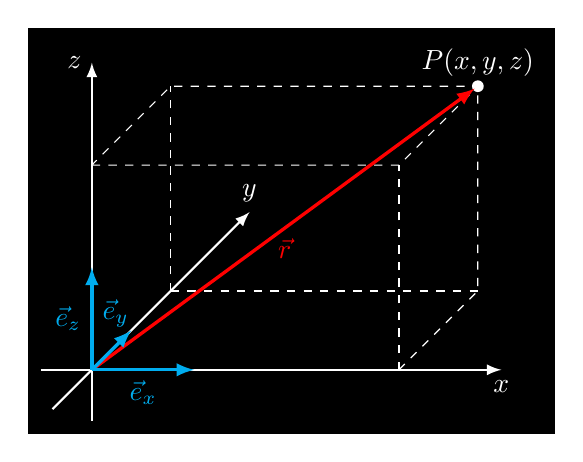
\begin{tikzpicture}[inverted,scale=1.3]
  % axes
  \draw[->,thick] (xyz cs:x=-0.5) -- (xyz cs:x=4)  node[below] {$x$};
  \draw[->,thick] (xyz cs:y=-0.5) -- (xyz cs:y=3)  node[left]  {$z$};
  \draw[->,thick] (xyz cs:z=1)    -- (xyz cs:z=-4) node[above] {$y$};
  % dashed lines
  \draw[dashed] (xyz cs:x=3)  -- ++(xyz cs:z=-2) -- ++(xyz cs:y=2) coordinate (p) node[above] {$P(x,y,z)$};
  \draw[dashed] (xyz cs:z=-2) -- ++(xyz cs:x=3);
  \draw[dashed] (xyz cs:x=0,y=2,z=0) -- ++(xyz cs:x=3) -- ++(xyz cs:z=-2) -- ++(xyz cs:x=-3) -- ++(xyz cs:z=2);
  \draw[dashed] (xyz cs:x=3)  -- ++(xyz cs:y=2);
  \draw[dashed] (xyz cs:z=-2) -- ++(xyz cs:y=2);
  \node[fill,circle,inner sep=1.5pt] at (p) {};
  % point
  \draw[->,very thick,red,shorten >= 0.5mm] (xyz cs:x=0) -- node[below]{$\place$} (xyz cs:x=3,y=2,z=-2);
  % unit vectors
  \draw[->,very thick,blue] (xyz cs:x=0) -- node[below]{$\ex$} (xyz cs:x=1);
  \draw[->,very thick,blue] (xyz cs:x=0) -- (xyz cs:z=-1) node[left,yshift=0.6em,xshift=0.3em]{$\ey$};
  \draw[->,very thick,blue] (xyz cs:x=0) -- node[left]{$\ez$} (xyz cs:y=1);
\end{tikzpicture}
\end{document}
